\section{Resultados de predição com o PSIPRED}

O PSIPRED é um método de predição de estruturas secundárias que utiliza redes neurais artificias em conjunto com PSSM \citep{10.1006/jmbi.1999.3091} (ver \ref{ch:rev_literatura}). O método foi originalmente treinado com informações da estrutura secundária atribuídas pelo DSSP. 

Devido as variações observadas entre os métodos de atribuição de estrutura secundária, nós realizamos a comparação dos resultados de predição com a estrutura secundária atribuída por diferentes métodos, assim como com o consenso entre os métodos de atribuição.

No conjunto de proteínas utilizado nesse trabalho, o PSIPRED comparado à atribuição pelo DSSP, demonstrou uma acurácia média (Q3) de 86\%, superior aos 78\% descrito na literatura. 

A acurácia média para a predição de fitas $\beta$, como esperado, foi inferior a predição de hélices e coils.

Um resultado interessante foi a acurácia média observada entre a predição e o consenso dos métodos de atribuição estrutura secundária. Tanto a acurácia geral (Q3) quantos a acurácia por classe (Qh, Qe, Qc) demonstraram aumentos significativo em comparação com os métodos de atribuição individuais. 

Isso indica que nas regiões onde não há consenso entre os métodos de atribuição, a acurácia média (Q3) é próxima ou inferior a 68\%.

$Q3_\text{consenso}*P_\text{consenso} + Q3_\text{não consenso}*P_\text{não consenso} = Q3_\text{total}$

$Q3_\text{não consenso} = \frac{Q3_\text{total} - Q3_\text{consenso}*P_\text{consenso}}{P_\text{não consenso}}$

$Q3_\text{não consenso} = \frac{0.86 - 0.92*0.75}{0.25}$

$Q3_\text{não consenso} = 0.68$

%Comentar que entre os piores resultados de acurácia há grande presença de zinc fingers resolvidas em complexo com o DNA. Discutir o sentido disso

\begin{figure}
    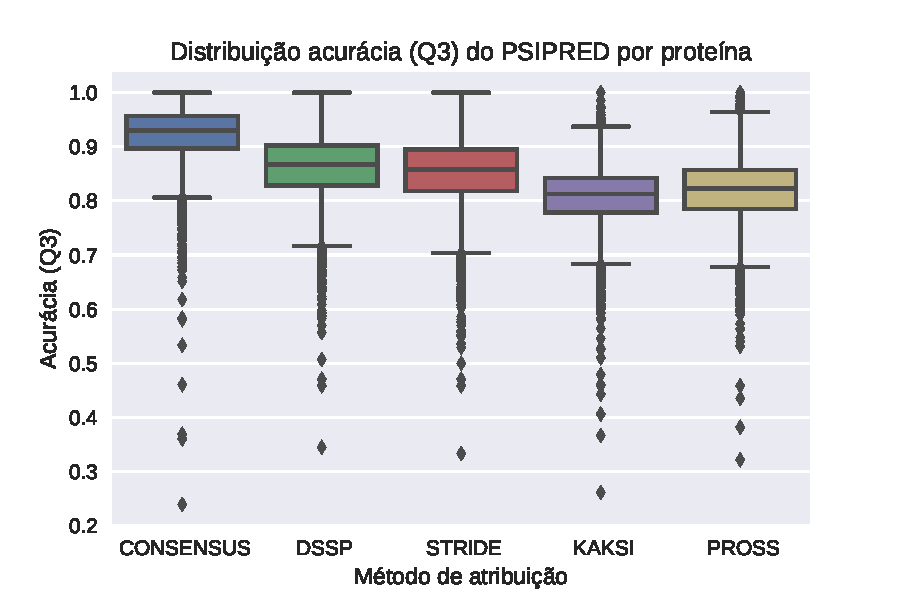
\includegraphics[width=\linewidth]{../figures/psipred_q3.pdf}
    \caption{}
    \label{fig:psipred_q3}
\end{figure}

\begin{figure}
    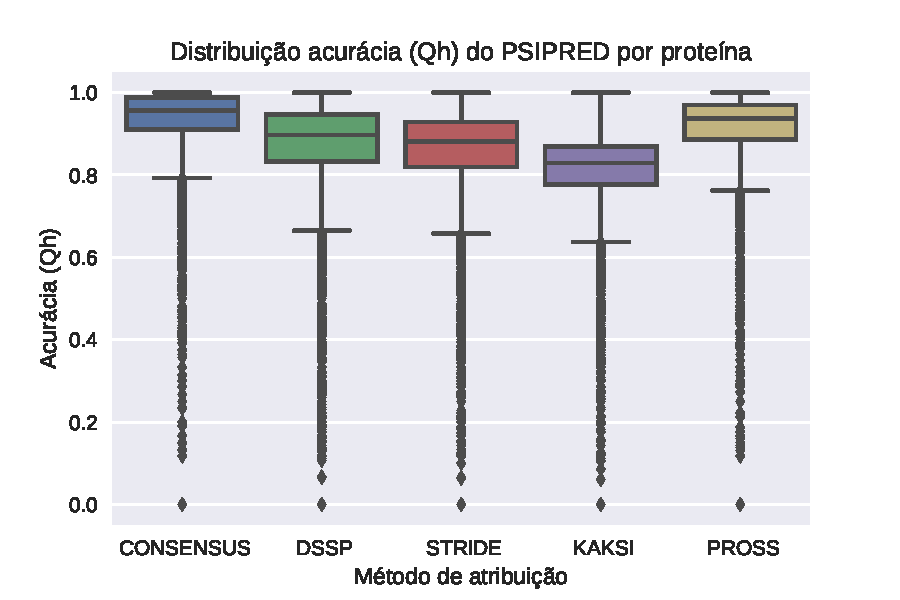
\includegraphics[width=\linewidth]{../figures/psipred_qh.pdf}
    \caption{}
    \label{fig:psipred_qh}
\end{figure}

\begin{figure}
    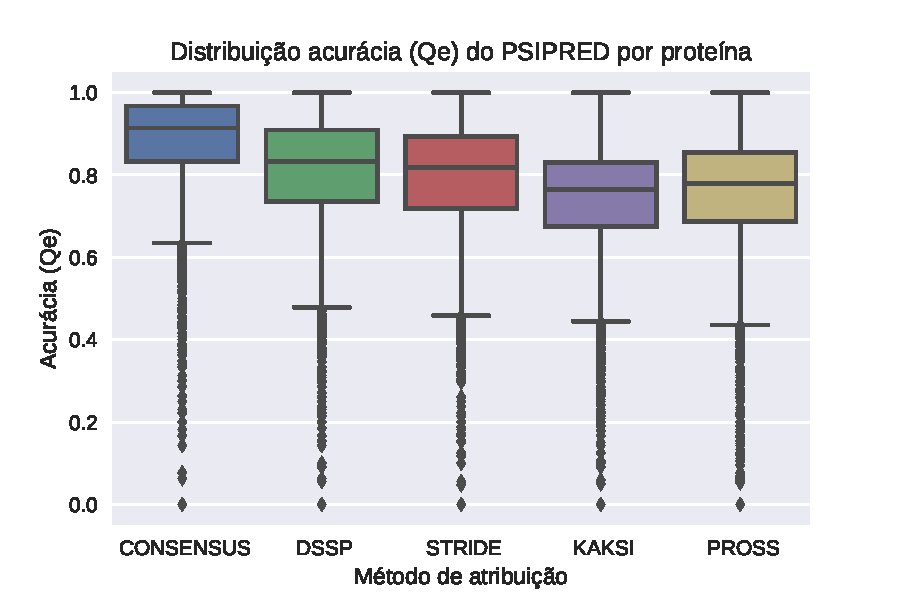
\includegraphics[width=\linewidth]{../figures/psipred_qe.pdf}
    \caption{}
    \label{fig:psipred_qe}
\end{figure}

\begin{figure}
    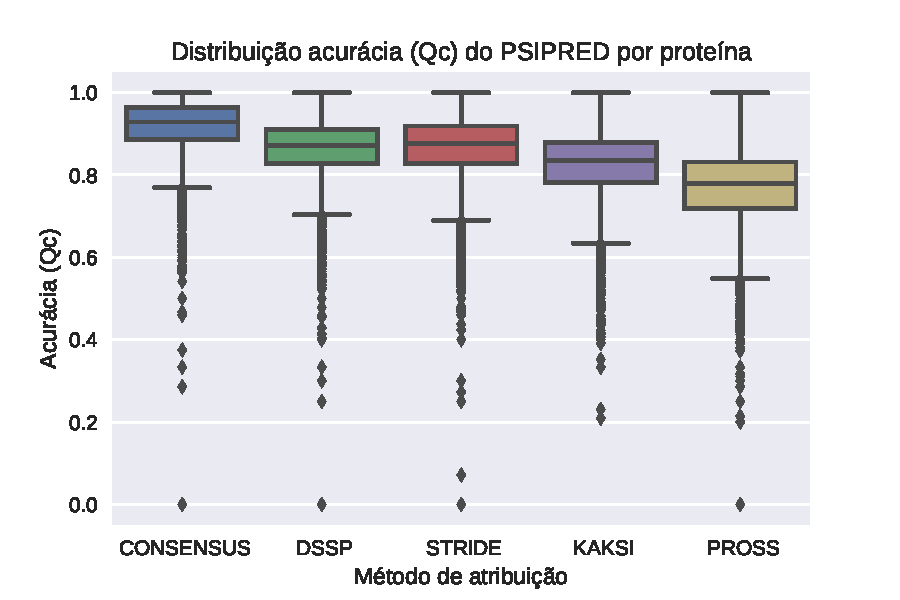
\includegraphics[width=\linewidth]{../figures/psipred_qc.pdf}
    \caption{}
    \label{fig:psipred_qc}
\end{figure}

\begin{figure}
    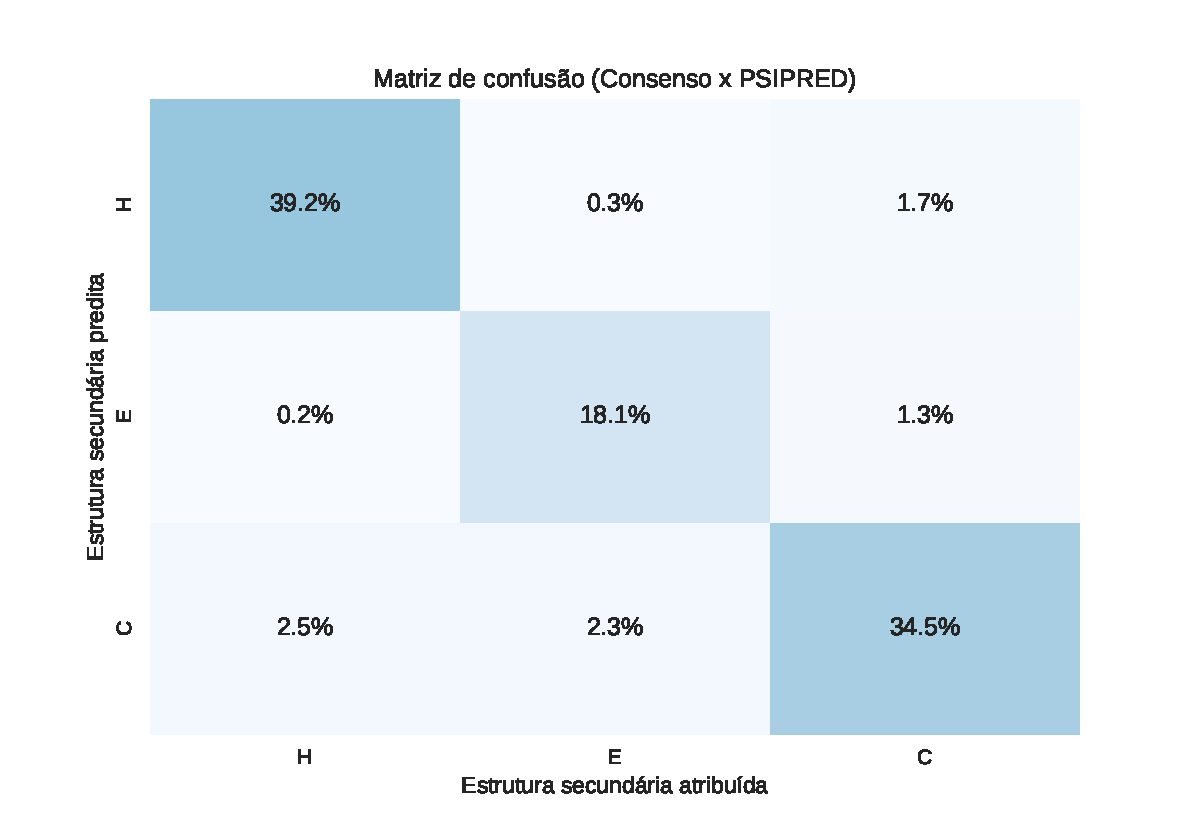
\includegraphics[width=\linewidth]{../figures/psipred_all3_confusion_matrix.pdf}
    \caption{}
    \label{fig:psipred_all3_confusion_matrix}
\end{figure}

\begin{figure}[ht] 
    \begin{subfigure}[b]{0.5\linewidth}
      \centering
      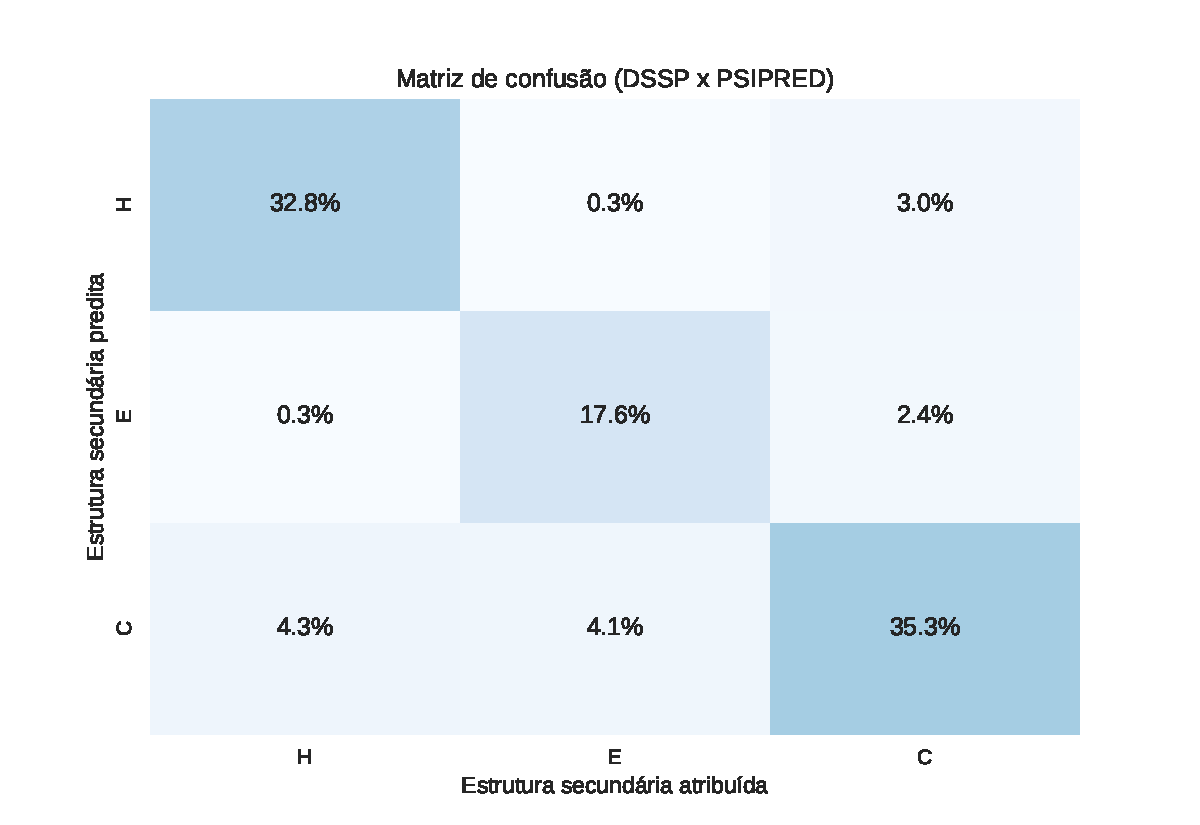
\includegraphics[width=1.0\linewidth]{../figures/psipred_dssp_confusion_matrix.pdf} 
      \caption{Initial condition} 
      \label{fig7:a} 
      \vspace{4ex}
    \end{subfigure}%% 
    \begin{subfigure}[b]{0.5\linewidth}
      \centering
      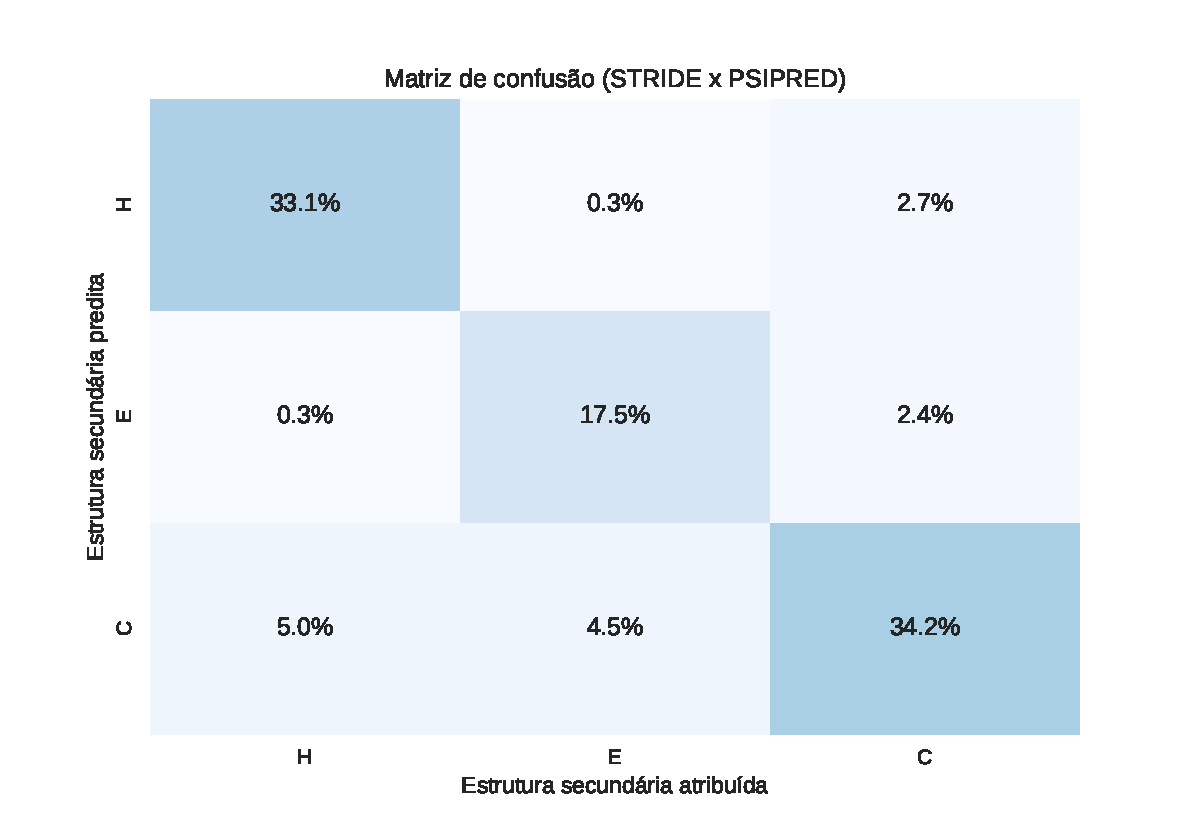
\includegraphics[width=1.0\linewidth]{../figures/psipred_stride_confusion_matrix.pdf} 
      \caption{Rupture} 
      \label{fig7:b} 
      \vspace{4ex}
    \end{subfigure} 
    \begin{subfigure}[b]{0.5\linewidth}
      \centering
      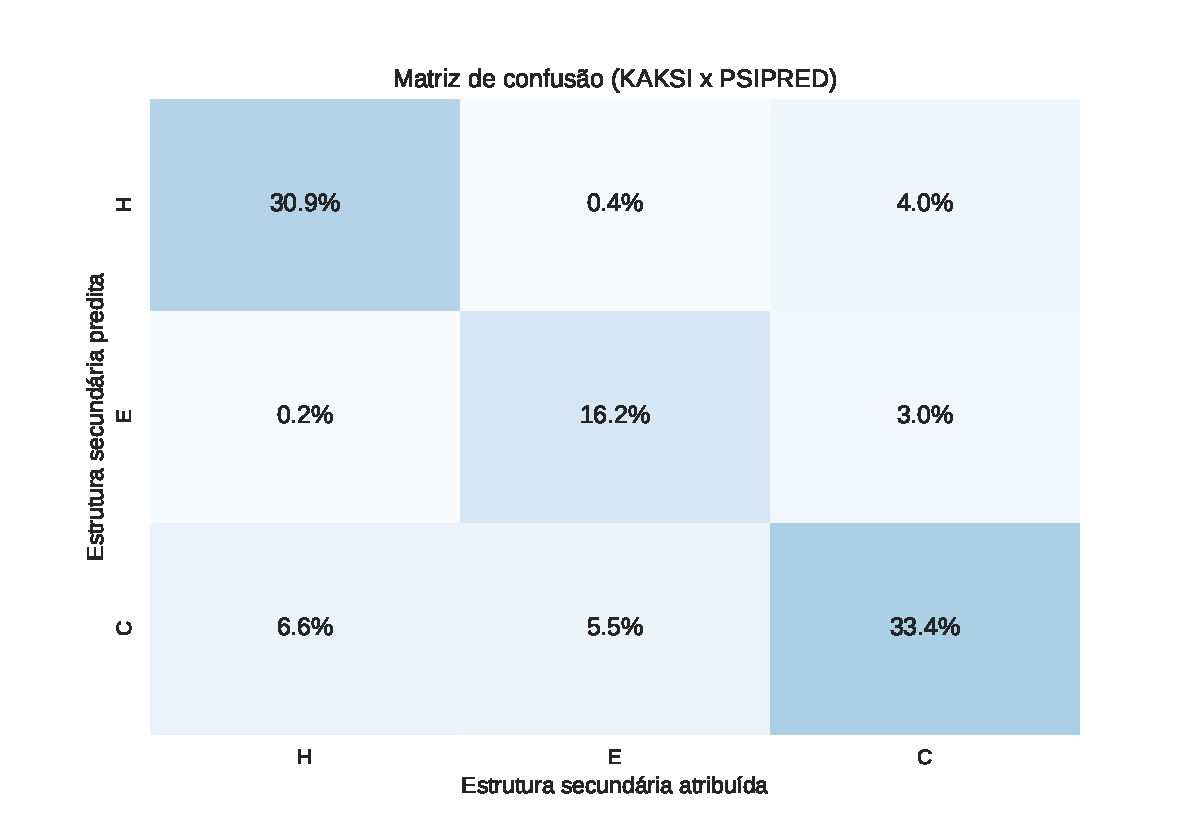
\includegraphics[width=1.0\linewidth]{../figures/psipred_kaksi_confusion_matrix.pdf} 
      \caption{DFT, Initial condition} 
      \label{fig7:c} 
    \end{subfigure}%%
    \begin{subfigure}[b]{0.5\linewidth}
      \centering
      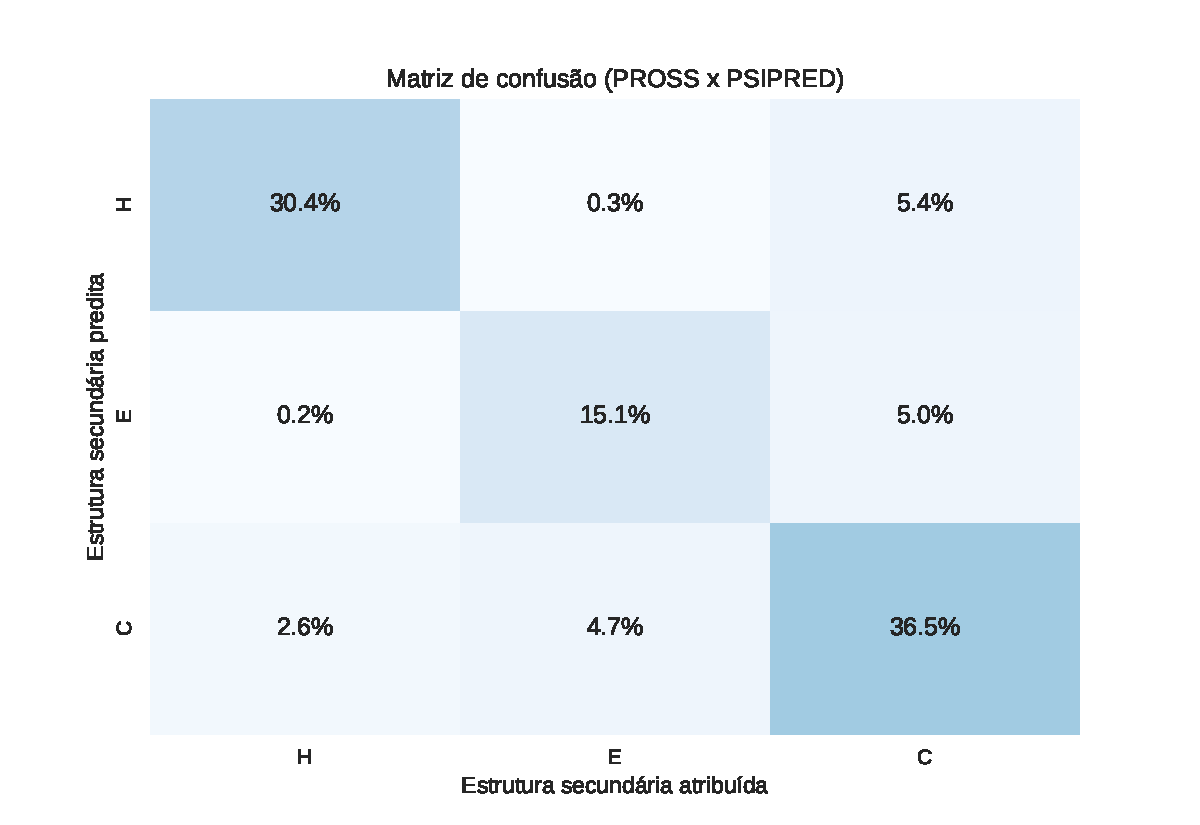
\includegraphics[width=1.0\linewidth]{../figures/psipred_pross_confusion_matrix.pdf} 
      \caption{DFT, rupture} 
      \label{fig7:d} 
    \end{subfigure} 
    \caption{Illustration of various images}
    \label{fig7} 
  \end{figure}